\chapter{Detection simulation}\label{ch:detection-simulation}

\section{Generation of EMRI LISA response}\label{sec:generation-of-emri-lisa-response}
Elaborate on \emph{FEW} \cite{Katz_2021,Chua_2021} and \emph{fastlisaresponse} \cite{Katz_2022} package.

\section{Detection of EMRI events}\label{sec:detection-of-emri-signals}
Given an EMRI LISA response in the form of the TDI channels $A,E$ and $T$, where $T$ corresponds to the \emph{null} or \emph{noise} channel and can therefore be neglected, we call it a detection if the optimal SNR is above the threshold $\text{SNR}_{\text{th}} = 20$. The optimal SNR is defined as
\begin{equation}
    \label{eq:optimal-snr}
    \begin{split}
        \text{SNR} &= \braket{h(t), h(t)}^{1/2}, \\
        &= \left( \int_{0}^{\infty} \frac{\abs{\tilde{h}(f)}^2}{S_n(f)} \, \text{d}f \right)^{1/2},
    \end{split}
\end{equation}
where $S_n(f)$ is the single-sided noise power spectral density (PSD) of the LISA detector. \emph{Single-sided} because it is obtained from integrating over the physical frequency range $[0, \infty)$. By construction, the TDI channels $A$ and $E$ are orthogonal with respect to the scalar product of real functions \fullref{eq:scalar-product-real-functions}, and therefore the optimal SNR is given by
\begin{equation}
    \label{eq:optimal-snr-tdi}
    \text{SNR} = \left( \int_{0}^{\infty} \frac{\abs{\tilde{h}_A(f)}^2 + \abs{\tilde{h}_E(f)}^2}{S_n(f)} \, \text{d}f \right)^{1/2}.
\end{equation}
Because the generation time of the LISA response scales with the observation time $\tobs$ as well as the SNR as can be seen in \fullref{fig:quick-snr-check-validation}, in the interest of computational efficiency, we introduce a first checkpoint called \emph{quick SNR check} where we compute the SNR for an observation time $\tobs = 1\unit{yr}$ and require $\text{SNR}_\text{th}^\text{quick} = 0.2 \cdot \text{SNR}_\text{th}$ to be exceeded. If this condition is met, we proceed to compute the optimal SNR for the full observation time $\tobs$ and compare it to the threshold $\text{SNR}_\text{th}$. If the full SNR is above the threshold, we consider the signal to be detected. This quick SNR check is a computationally efficient way to filter out signals that are extremely unlikely to be detected. Once we have detected a signal, we can proceed to compute the Cramér-Rao bounds on the parameters of the EMRI signal.

\begin{figure}
    \centering
    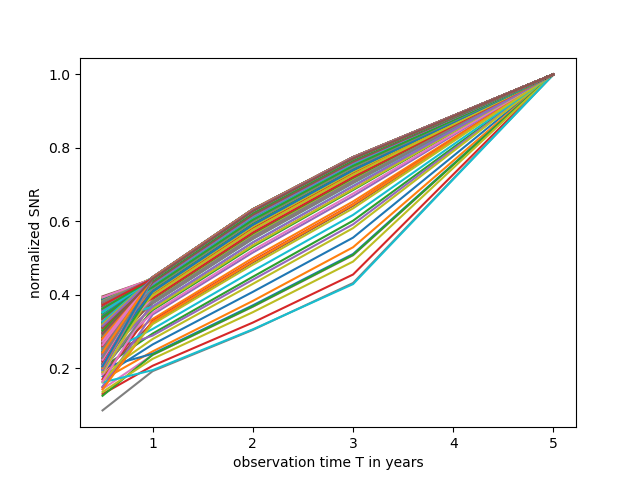
\includegraphics[width=0.49\textwidth]{SNR_observation_time.png}
    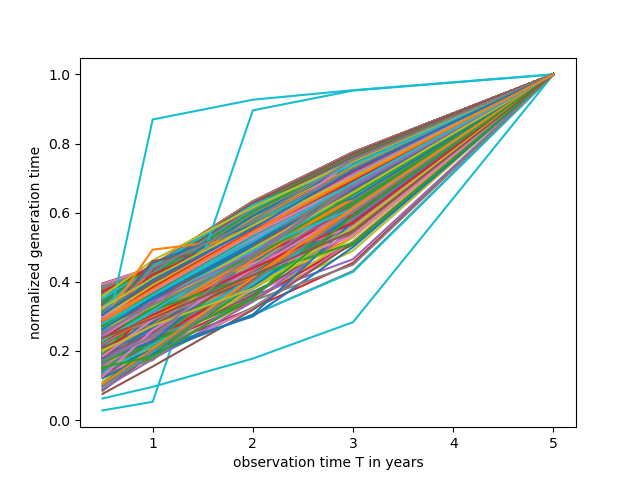
\includegraphics[width=0.49\textwidth]{generation_time_observation_time.png}
    \caption[Validation of quick SNR check]{On the left the optimal SNR as a function of observation time $\tobs$ for a large set of EMRI signals with randomly chosen parameters is shown. On the right we plot the generation time of the LISA response as a function of observation time $\tobs$ for the same set of EMRI signals. We choose a threshold of $\text{SNR}^{\text{quick}}_\text{th} = 0.2 \cdot \text{SNR}_\text{th}$ for the quick SNR check.}
    \label{fig:quick-snr-check-validation}
\end{figure}

\subsection{Computing Cramér-Rao bounds}\label{subsec:cramer-rao-bound}
As introduced in \fullref{ch:parameter-estimation}, the Cramér-Rao bounds $\bm{\Sigma}_\text{CR}$, i.e. lower limits for the covariance matrix, for the limit of high SNR are given by the inverse of the Fisher information matrix $\bm{\Gamma}^{-1}$. Thus, we need to compute the Fisher information matrix $\bm{\Gamma}$ (\fullref{eq:fisher-information-matrix}) for the EMRI signal, i.e. evaluate the derivatives of the waveform $\partial_{\theta^i} h(t; \theta)$ with respect to the 15 parameters $\theta$ of an EMRI event. We use the finite difference method
\begin{equation}
    \label{eq:finite-difference}
    \partial_{\theta^i} h(t; \theta) \approx \frac{h(t; \theta^i + \varepsilon) - h(t; \theta^i)}{\varepsilon},
\end{equation}
where $\varepsilon = 10^{-6}$ and $\theta$ are the simulation parameters that were used to generate the EMRI LISA response. We omitted the rest of the parameters in the notation for clarity. We can then use the derivatives to compute the components fo the Fisher information matrix via the scalar product of functions \fullref{eq:scalar-product-real-functions} and store the Cramér-Rao bounds. In this fashion we create a collection of EMRI signals that were detected and for which we have computed the Cramér-Rao bounds on the parameters.

\section{Numerical bottlenecks}\label{sec:numerical-bottlenecks}
\subsection{Generation of the EMRI LISA response}\label{subsec:generation-of-the-emri-lisa-response}
For the simulation of the EMRI detections, the important consideration for the computational cost is the generation of the waveform which is, thanks to the GPU parallelization, already very fast (see \fullref{fig:waveform-generation-time}) with an average computation time of $0.933$s. Nevertheless, this will become a bottleneck if we start using more accurate approximation when computing the derivative such as the five point stencil method that uses five evaluations of the waveform for each of the 15 parameters. This is why for now the simulation uses the finite difference method \fullref{eq:finite-difference} to compute the derivatives. [TODO: error estimation for derivatives]
\begin{figure}
    \centering
    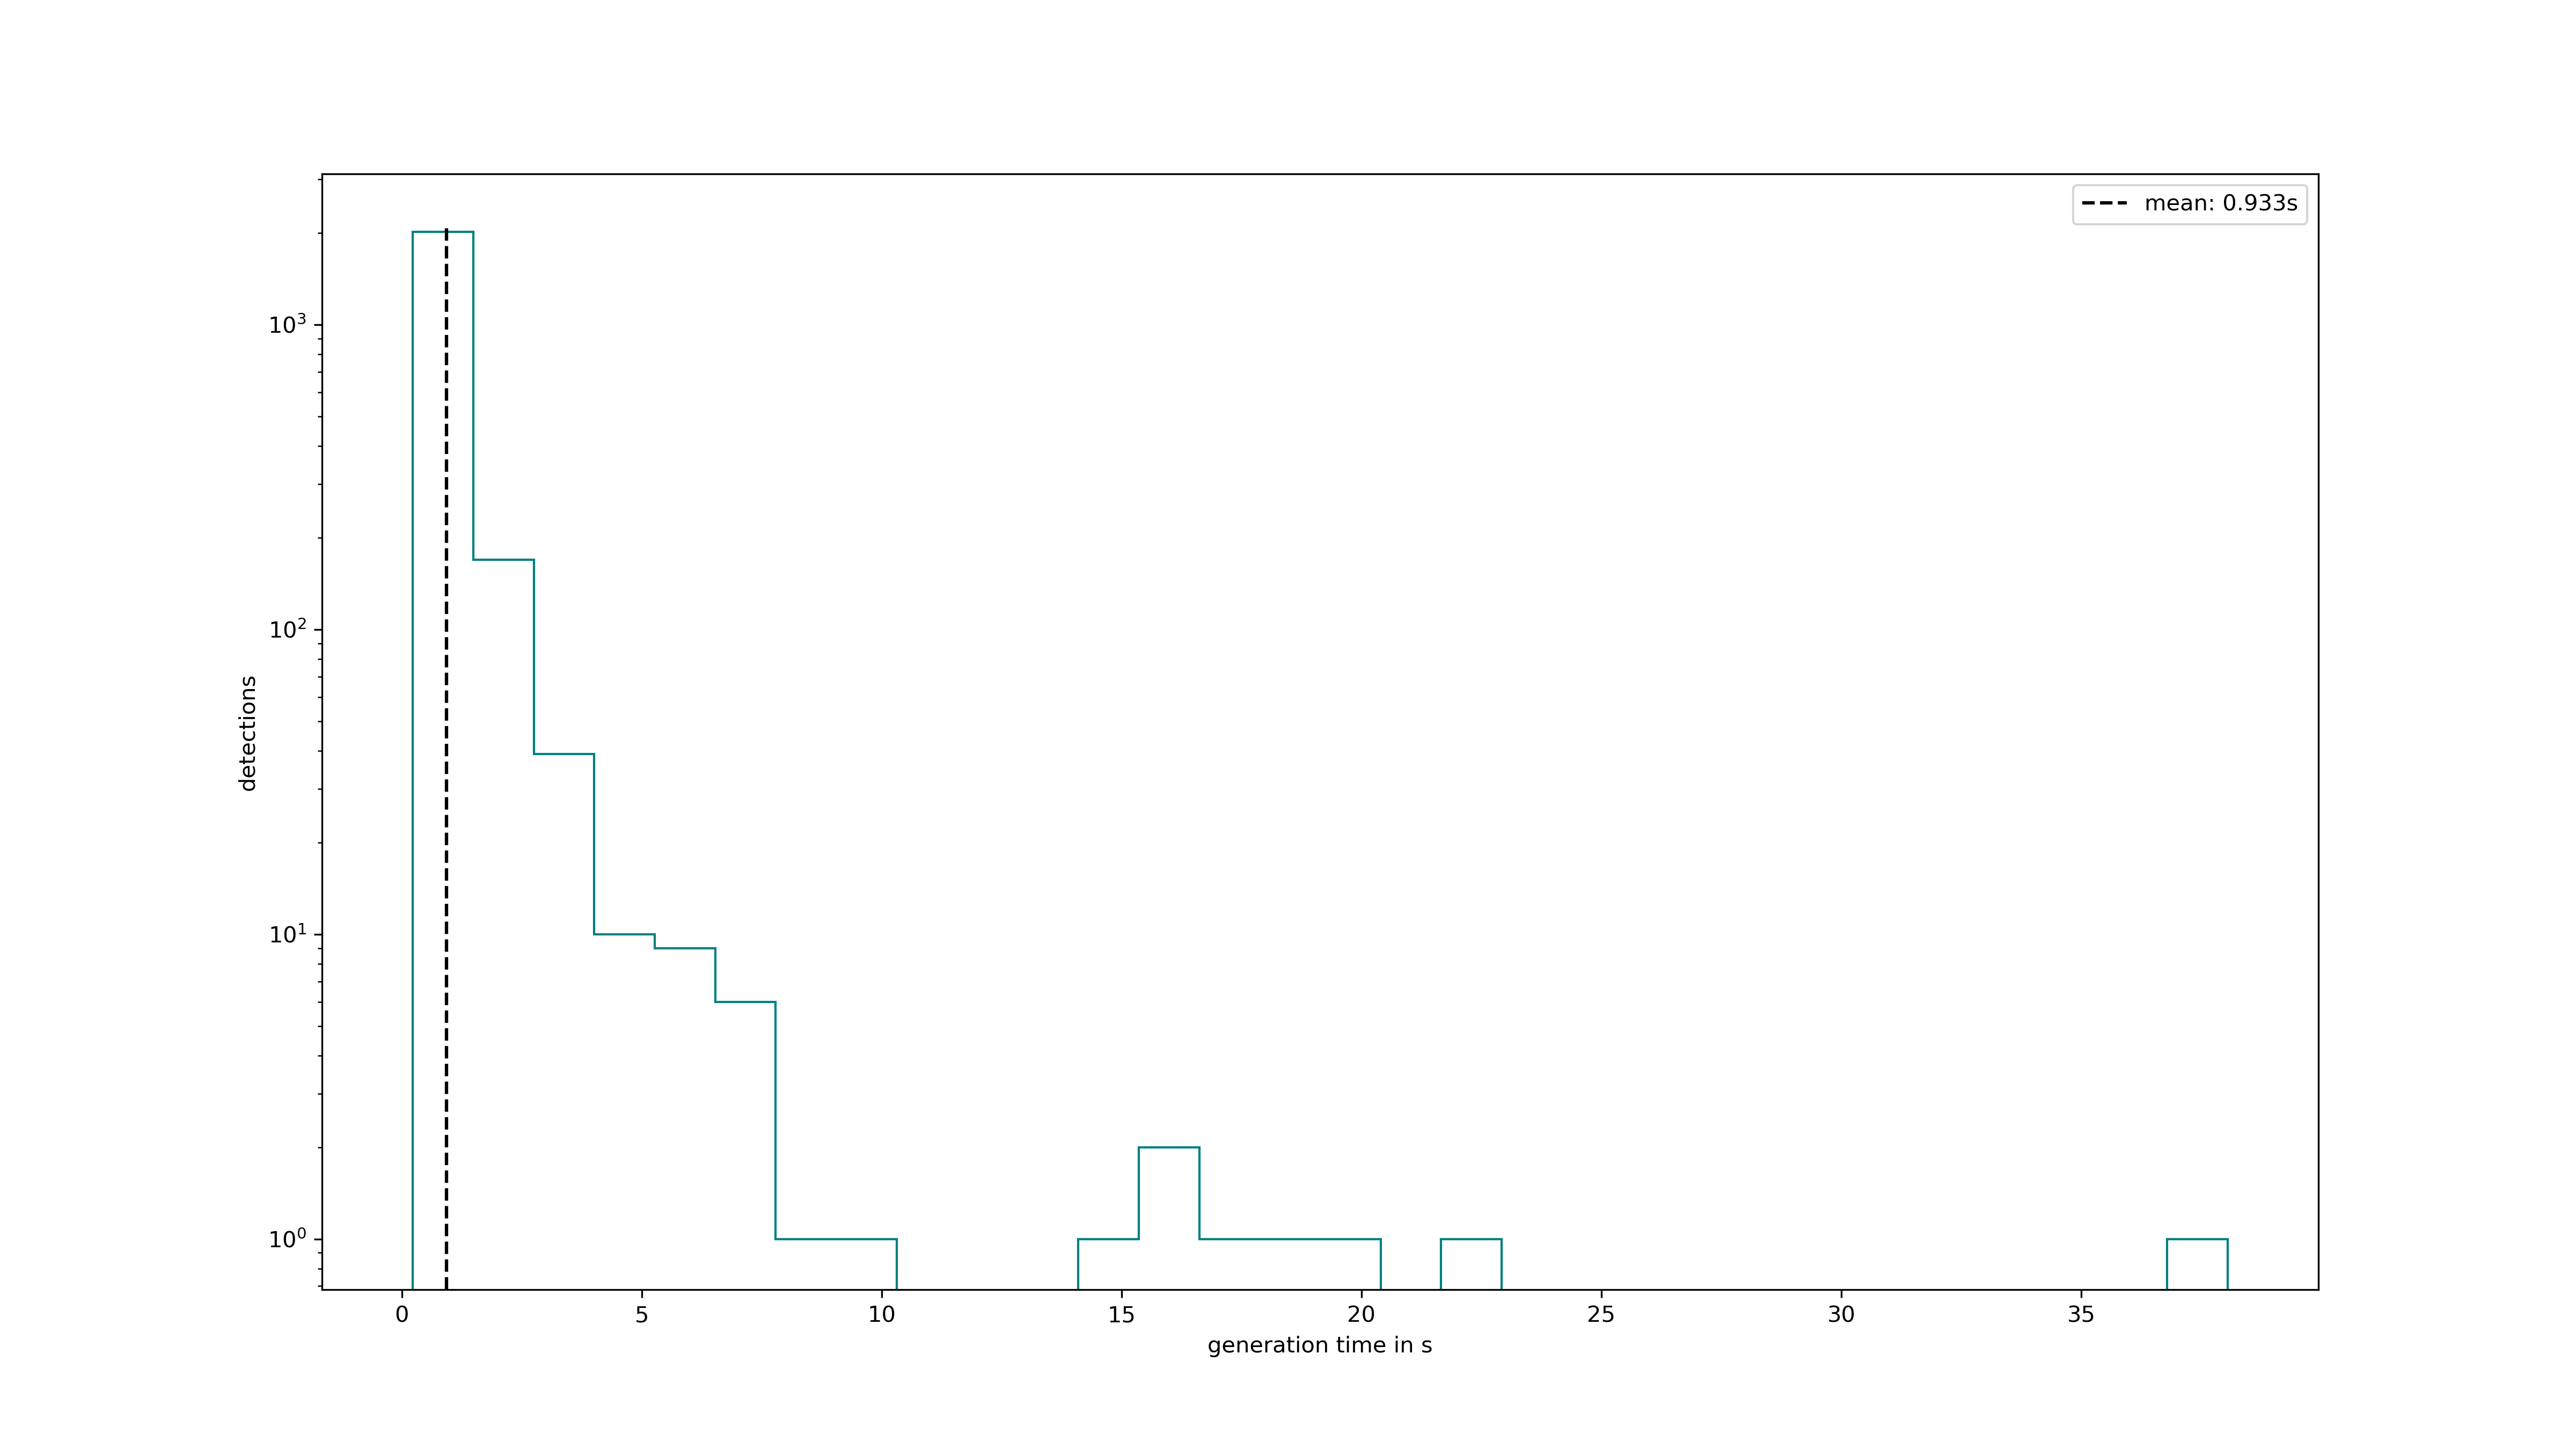
\includegraphics[width=0.8\textwidth]{generation_time.png}
    \caption[Waveform generation time histogram]{Histogram of the generation time of the EMRI LISA response using the python modules \emph{fastlisaresponse} and \emph{FEW}.}
    \label{fig:waveform-generation-time}
\end{figure}

\subsection{Computation of the posterior}\label{subsec:computing-the-fisher-information-matrix}
The computation of the posterior distribution has to be done for every value of $\rhubble$ in the discretized interval $[0.6, 0.86]$. For each value of $\rhubble$ we then iterate over all detections and have to compute the likelihood of each galaxy for given detection and given value of $\rhubble$. As the galaxies are weighted by the gaussian distributions in …\fullref{eq:likelihood-final}, we can reduce the sum over all galaxies in the catalog to a sum over all galaxies within an error volume defined by the detection parameter uncertainties. We use a $3 \sigma$ cutoff for the error volume, e.g. [$\hat{\varphi} - 3 \sigma_\varphi$, $\hat{\varphi} + 3 \sigma_\varphi$] for the parameter $\varphi$. Further, instead of considering the full range in redshift when integrating over $\zgw$ in \fullref{eq:likelihood-final}, we can set outer bounds $z_\text{min}, z_\text{max}$ using the prior we imposed on the range of $\rhubble$ to compute
\begin{equation}
    \label{eq:redshft-outer-bounds}
    \begin{split}
        z_\text{min} &= z(\hat{\dl} - 4\sigma_{\dl}, \rhubble_\text{min}), \\
        z_\text{max} &= z(\hat{\dl} + 4\sigma_{\dl}, \rhubble_\text{max}),
    \end{split}
\end{equation}
where $z(\dl, \rhubble)$ is the inverse of the luminosity distance function \fullref{eq:luminosity-distance}.
For the detections evaluated in \fullref{ch:galaxy-catalog-as-ground-truth} the number of possible hosts are shown in \fullref{fig:possible-hosts}. Last but not least, we take a look at the integral over $\Mbh$ in \fullref{eq:likelihood-final}. Let us first isolate the part of the integral that depends on $\Mbh$
\begin{equation}
    p(\detection |\rhubble , \galcat , \cosmologicalmodel, \backgroundinformation) \propto \int \dd \Mbh g(\Mbh) \cdot \exp \left \{ -\frac{(\hat{\Mz} - \Mbh (1 + \zgw))^2}{2 \sigma_{\Mz}^2}  \right \},
\end{equation}
where $g(\Mbh)$ are the covariance contributions and the normal distribution $\normaldist{\Mbh^{(k)}}$ terms that depend on $\Mbh$. If we compare the relative error of $\Mz$ for detections  and the galaxy catalog in \fullref{fig:relative-mass-error-distribution}, we see that the relative error is a lot smaller for the detections
\begin{equation}
    \label{eq:relative-mass-error}
    \begin{split}
        \sfrac{\sigma_{\Mz}}{\hat{\Mz}} &\le 10^{-6}, \quad \forall \detection \in \detections \\
        \sfrac{\sigma_{\Mbh}}{\Mbh} &\ge 0.2, \quad \forall \galaxy \in \galcat.
    \end{split}
\end{equation}
Hence, we can treat the exponential term effectively as a delta function and reduce the integral to
\begin{equation}
    \begin{split}
        p(\detection |\rhubble , \galcat , \cosmologicalmodel, \backgroundinformation) &\propto \int \dd \Mbh g(\Mbh) \cdot \delta (\hat{Mz} - \Mbh (1 + \zgw)) \\
        &= \frac{g(\frac{\hat{\Mz}}{1 + \zgw})}{1 + \zgw},
    \end{split}
\end{equation}
where we used to representation of the delta function
\begin{equation}
    \delta(x) = \lim_{\varepsilon \rightarrow 0} \frac{1}{\sqrt{2\pi \varepsilon}} \exp \left \{ -\frac{x^2}{2 \varepsilon} \right \}
\end{equation}
and its property
\begin{equation}
    \int \dd x g(x) \delta(f(x)) = \sum_{x_i} \frac{g(x_i)}{\abs{f'(x_i)}},
\end{equation}
where $x_i$ are the roots of $f(x) = 0$.

\section{Bias correction}\label{sec:bias-correction}
The way we



\begin{figure}
    \centering
    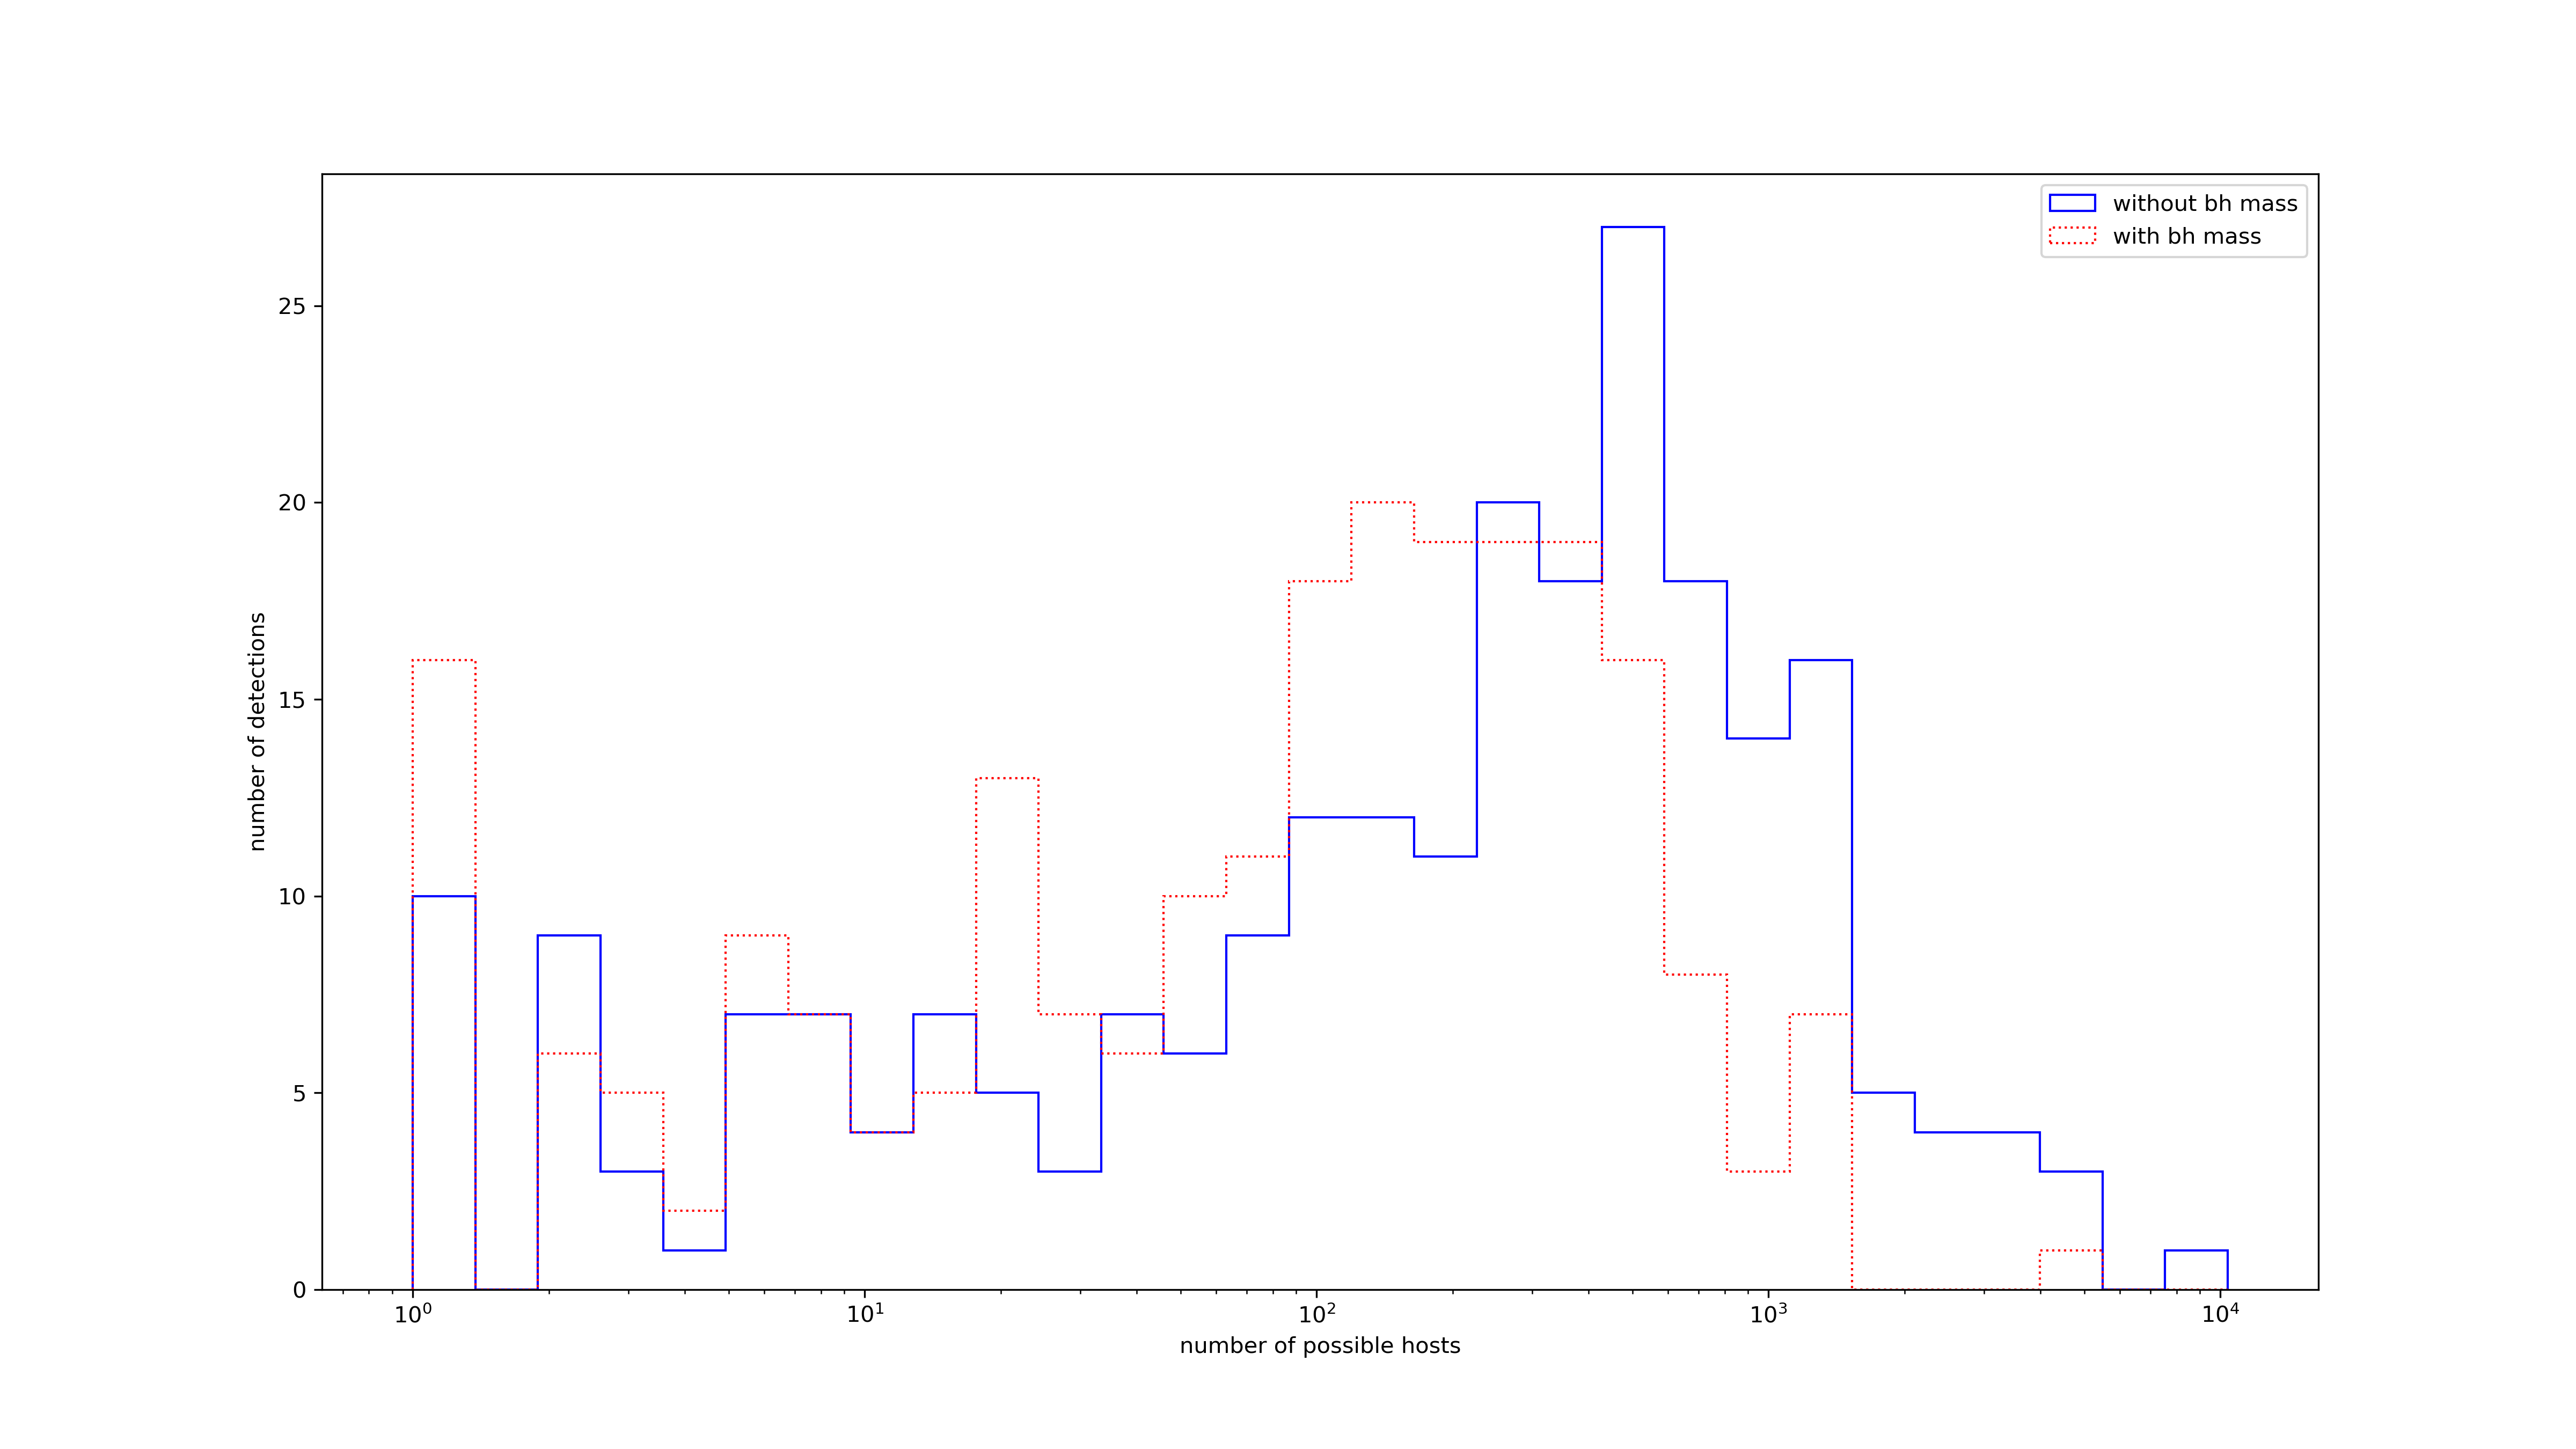
\includegraphics[width=0.8\textwidth]{number_of_possible_hosts.png}
    \caption[Number of possible hosts]{Number of possible hosts for each detection using a $3\sigma$ region on the considered parameters.}
    \label{fig:possible-hosts}
\end{figure}

\begin{figure}
    \centering
    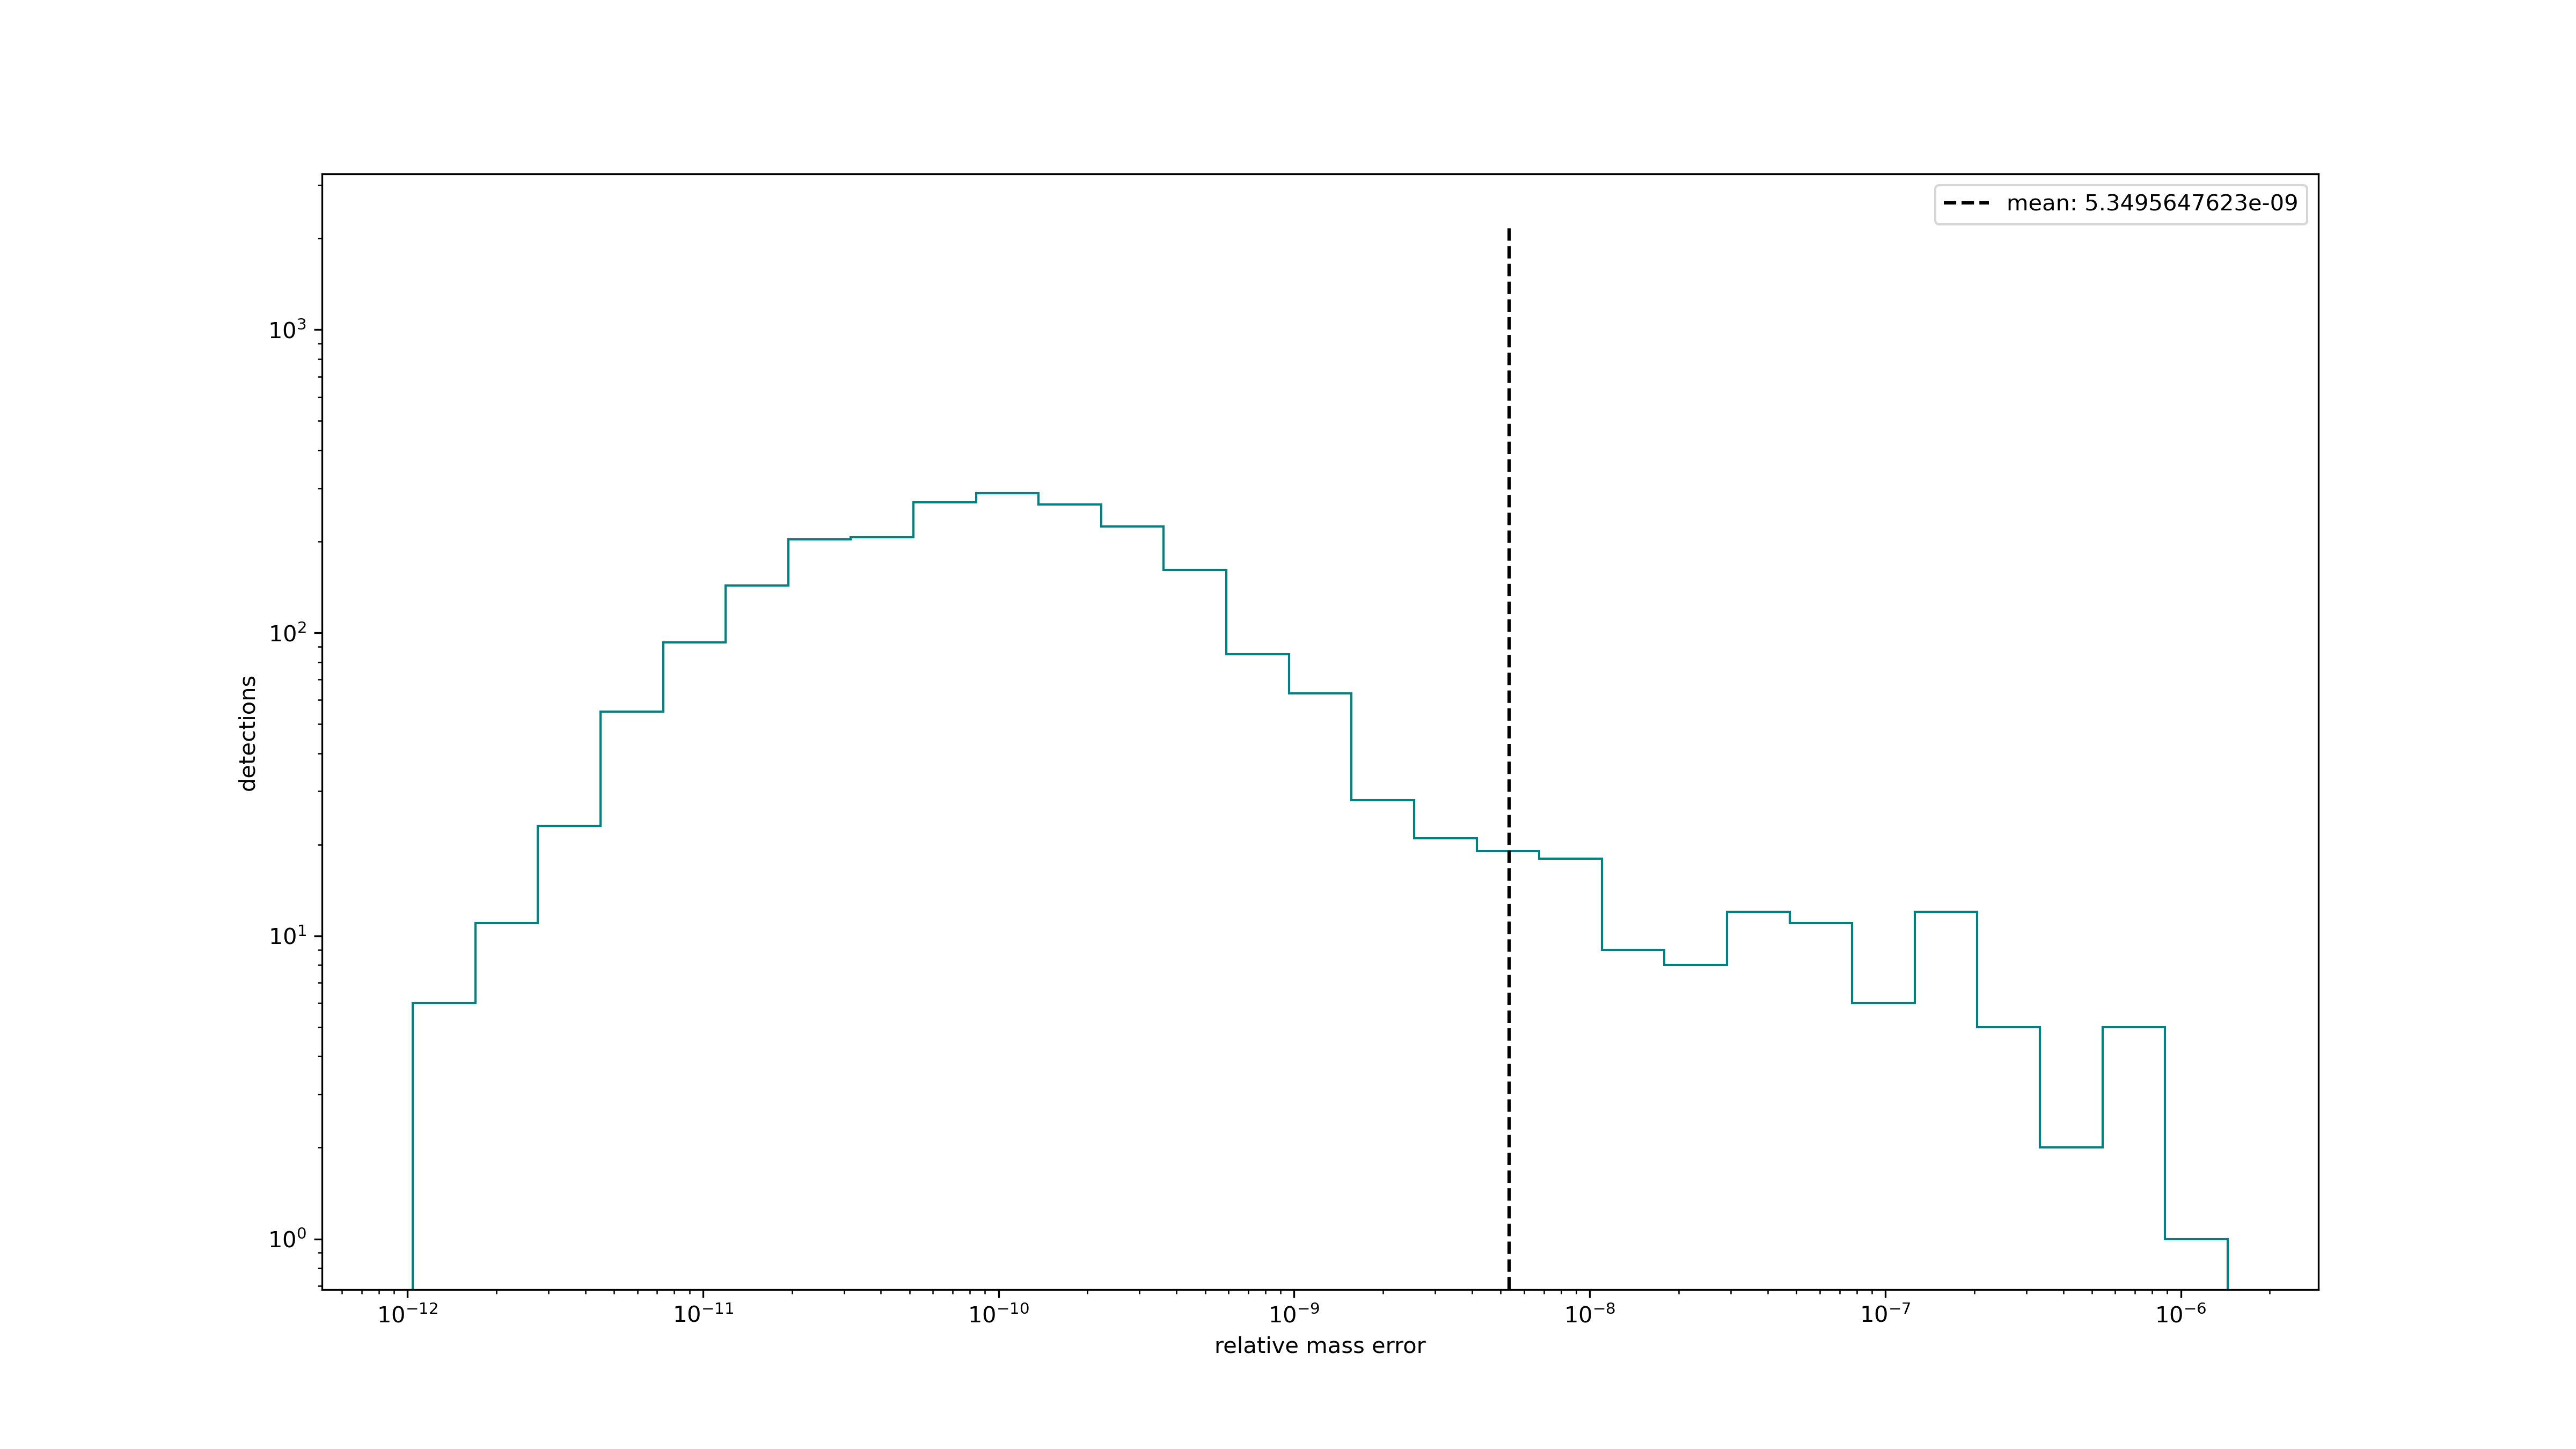
\includegraphics[width=0.49\textwidth]{relative_mass_error.png}
    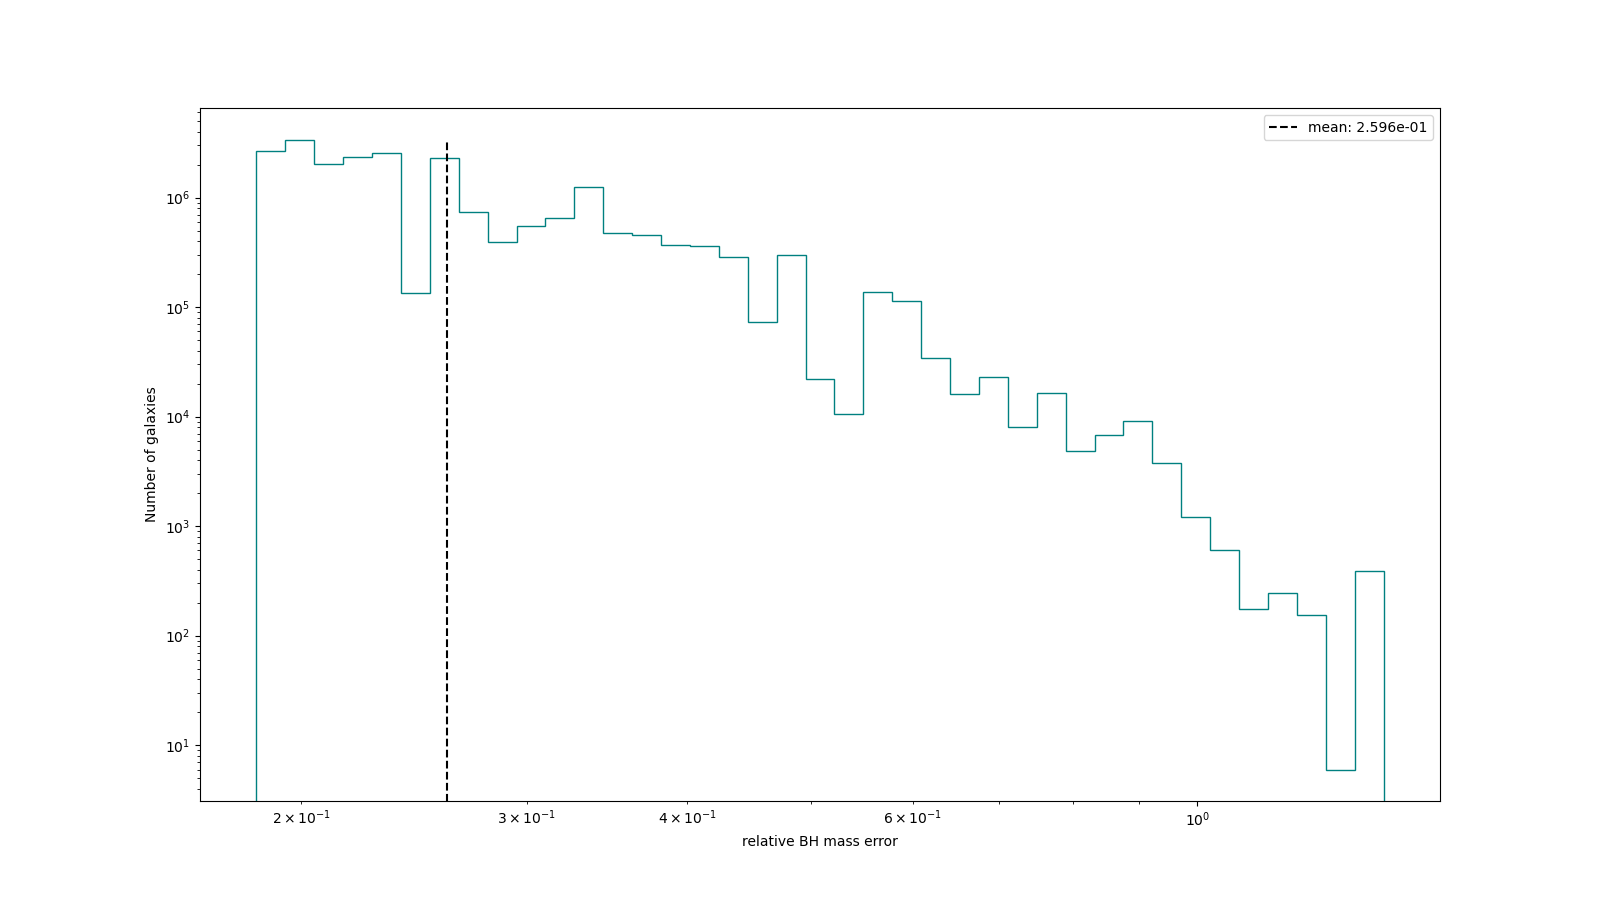
\includegraphics[width=0.49\textwidth]{relative_BH_mass_error_distribution.png}
    \caption[Relative mass error detection and galaxy catalog]{Left: relative mass error histogram for detections used in \fullref{ch:galaxy-catalog-as-ground-truth}. Right: relative mass error distribution for the galaxy catalog.}
    \label{fig:relative-mass-error-distribution}
\end{figure}


